\documentclass[tikz,border=10pt]{standalone}
\usepackage{pgfplots}
\usepgfplotslibrary{fillbetween}
\pgfplotsset{compat=1.18}

\begin{document}

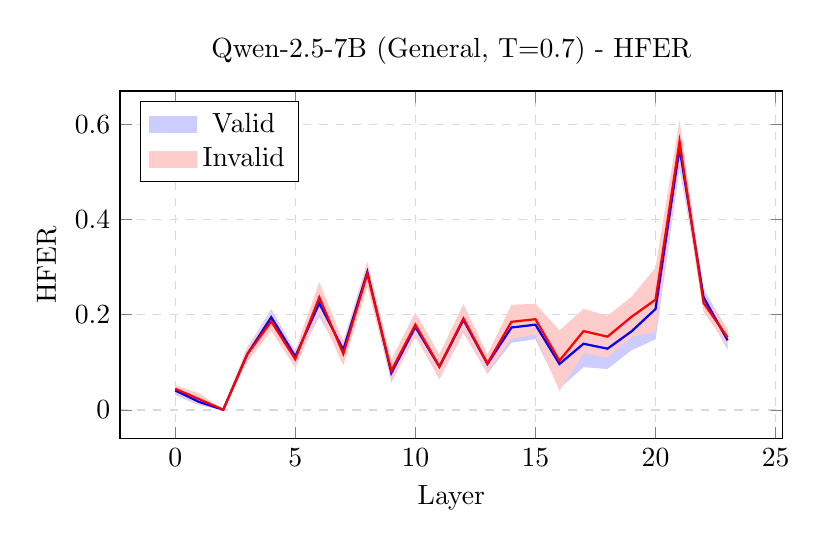
\begin{tikzpicture}
\pgfplotstableread[row sep=newline, col sep=comma]{
layer,v_mean,v_std,i_mean,i_std,v_upper,v_lower,i_upper,i_lower

0,0.04103623577393587,0.00945393601949947,0.04452381320297714,0.00755298108811733,0.05049017179343534,0.0315822997544364,0.052076794291094464,0.03697083211485981

1,0.0168057002476416,0.006858831358791826,0.022610026295296806,0.012220002589119443,0.023664531606433427,0.009946868888849776,0.03483002888441625,0.010390023706177363

2,0.0004272989545824663,0.00017972530362198987,0.0005724141112295351,0.0003121788343685989,0.0006070242582044561,0.00024757365096047645,0.0008845929455981339,0.0002602352768609362

3,0.1170213477686047,0.013505434306837136,0.11666941978037353,0.01567331233441262,0.13052678207544183,0.10351591346176757,0.13234273211478614,0.10099610744596091

4,0.1949161820113659,0.016894642065833843,0.18591360375285143,0.02003264938217562,0.21181082407719976,0.17802153994553205,0.20594625313502704,0.16588095437067582

5,0.11247529685497279,0.011196872060105641,0.106653019785881,0.017735674074129206,0.12367216891507843,0.10127842479486715,0.12438869386001021,0.08891734571175179

6,0.224033616296947,0.02851065368914416,0.23657556027173995,0.03212926410319073,0.2525442699860912,0.19552296260780286,0.2687048243749307,0.20444629616854923

7,0.12643335480242962,0.017606971879400343,0.11807398274540899,0.024521077158778153,0.14404032668182998,0.10882638292302928,0.14259505990418714,0.09355290558663085

8,0.28977114222943784,0.016250170464466685,0.2857192002236843,0.026438901210582857,0.30602131269390453,0.27352097176497114,0.31215810143426714,0.25928029901310146

9,0.07754298639483745,0.02039398562456914,0.08248073775321241,0.023254448116416866,0.09793697201940658,0.05714900077026831,0.10573518586962927,0.05922628963679554

10,0.1744140001013875,0.015446426805570729,0.1792530290782451,0.02566702251312218,0.18986042690695823,0.15896757329581676,0.20492005159136728,0.15358600656512295

11,0.09075092985294755,0.0258837615594226,0.09127341322600838,0.02496959893134216,0.11663469141237015,0.06486716829352496,0.11624301215735053,0.06630381429466622

12,0.18921255171298978,0.02627978460832598,0.19213172197341916,0.03045425578178612,0.21549233632131576,0.1629327671046638,0.22258597775520528,0.16167746619163303

13,0.09658601447008545,0.020481460995874622,0.09767468646168705,0.01801622614159056,0.11706747546596008,0.07610455347421083,0.1156909126032776,0.07965846032009649

14,0.17316667502745986,0.03201461096434614,0.18517992384731766,0.035707035597374454,0.205181285991806,0.14115206406311373,0.2208869594446921,0.1494728882499432

15,0.17908516861498355,0.030428073082987762,0.19064642563462253,0.03242452235331223,0.2095132416979713,0.1486570955319958,0.22307094798793475,0.1582219032813103

16,0.09661980387754734,0.05173461502191238,0.10348681276664133,0.06355757307368572,0.14835441889945972,0.044885188855634965,0.16704438584032705,0.039929239692955615

17,0.13907712316140527,0.04917592097850958,0.16561746820807452,0.04666336265883759,0.18825304413991484,0.0899012021828957,0.2122808308669121,0.11895410554923694

18,0.12872581901028748,0.04272535523770032,0.15395404361188408,0.04390778170039381,0.1714511742479878,0.08600046377258716,0.1978618253122779,0.11004626191149028

19,0.165005015861243,0.03969344235010041,0.19569612294435496,0.041876565884363046,0.20469845821134341,0.12531157351114258,0.23757268882871801,0.1538195570599919

20,0.21202349066734313,0.06361148884933059,0.23166455253958698,0.06727364254026472,0.2756349795166737,0.14841200181801256,0.2989381950798517,0.16439090999932227

21,0.5494096972048282,0.041872070747403886,0.564107047021389,0.0449471812876171,0.5912817679522321,0.5075376264574244,0.6090542283090061,0.5191598657337719

22,0.2367506893351674,0.017941501427776004,0.22483687028288837,0.017917083596819258,0.2546921907629434,0.2188091879073914,0.24275395387970763,0.2069197866860691

23,0.14621232235804196,0.019942339002473653,0.15237068310379978,0.018829209963291186,0.16615466136051563,0.1262699833555683,0.17119989306709096,0.1335414731405086

}\mydata

\begin{axis}[
    width=10cm, height=6cm,
    xlabel={Layer},
    ylabel={HFER},
    title={Qwen-2.5-7B (General, T=0.7) - HFER},
    legend pos=north west,
    grid=major,
    grid style={dashed, gray!30}
]

\addplot [name path=v_upper, draw=none, forget plot] table [x=layer, y=v_upper] {\mydata};
\addplot [name path=v_lower, draw=none, forget plot] table [x=layer, y=v_lower] {\mydata};
\addplot [blue!20] fill between [of=v_upper and v_lower];

\addplot [name path=i_upper, draw=none, forget plot] table [x=layer, y=i_upper] {\mydata};
\addplot [name path=i_lower, draw=none, forget plot] table [x=layer, y=i_lower] {\mydata};
\addplot [red!20] fill between [of=i_upper and i_lower];

\addplot [blue, thick] table [x=layer, y=v_mean] {\mydata};
\addlegendentry{Valid}
\addplot [red, thick] table [x=layer, y=i_mean] {\mydata};
\addlegendentry{Invalid}

\end{axis}
\end{tikzpicture}
\end{document}
